\documentclass[12pt,a4paper]{article}
% Change "article" to "report" to get rid of page number on title page
\usepackage{amsmath,mathtools,amsfonts,amsthm,amssymb}
\usepackage{setspace}
\usepackage{Tabbing}
\usepackage{fancyhdr}
\usepackage{lastpage}
\usepackage{extramarks}
\usepackage{chngpage}
\usepackage{fourier}
\usepackage{soul,color}
\usepackage[usenames,dvipsnames]{xcolor}
\usepackage{graphicx,float,wrapfig}
\usepackage[utf8]{inputenc}
\usepackage{sidecap}
\usepackage{marvosym}
\usepackage{tikz, tikz-qtree}
\usepackage{tabularx, multirow}
\usepackage{enumerate}
\usepackage{hyperref}
\definecolor{gray99}{gray}{.99}
\usepackage{listings}
\usepackage[english]{babel}
\usepackage{placeins}
\usepackage{tikz}
\usepackage{tikz-qtree}
\usepackage{xspace}
\usepackage{mathtools}
\usepackage{tabulary}
\lstset{
	language=R,
	backgroundcolor=\color{gray99},
	tabsize=3,
	frame=single,
	keywordstyle=\ttfamily\bfseries\color{RoyalBlue},
	commentstyle=\ttfamily\color{ForestGreen},
	stringstyle=\ttfamily\color{Gray},
	breaklines=true,
	showstringspaces=false,
	basicstyle=\footnotesize\ttfamily,
	emph={label},
	xleftmargin=22pt,
	framexleftmargin=22pt,
	framexrightmargin=0pt,
	framexbottommargin=4pt,
	numbers=left,
	stepnumber=1
}
\usepackage{caption}
\DeclareCaptionFont{black}{\color{black}}{\bfseries}
\DeclareCaptionFormat{listing}{\parbox{\textwidth}{\hspace{8pt}#1#2#3}}
\captionsetup[lstlisting]{format=listing,labelfont=black,textfont=black, singlelinecheck=false, margin=0pt, font={bf,footnotesize}}

% In case you need to adjust margins:
\topmargin=-0.45in      %
\evensidemargin=0in     %
\oddsidemargin=0in      %
\textwidth=6.5in        %
\textheight=9.5in       %
\headsep=0.25in         %

% Special font
\newcommand{\cps}[2]{\ensuremath{[[{#1}]]_{\textstyle #2}}}

% Homework Specific Information
\newcommand{\hmwkTopic}{MOOC Data Analysis}
\newcommand{\hmwkTitle}{Final Project - \hmwkTopic}
\newcommand{\hmwkDueDate}{May 16, 2014}
\newcommand{\hmwkClass}{CS 199}
\newcommand{\hmwkAuthorNameA}{Sam Laane}
\newcommand{\hmwkAuthorEmailA}{laane2@illinois.edu}
\newcommand{\hmwkAuthorNameB}{José Vicente Ruiz}
\newcommand{\hmwkAuthorEmailB}{ruizcep2@illinois.edu}
\newcommand{\hmwkAuthorNameC}{Nick Jeffrey}
\newcommand{\hmwkAuthorEmailC}{njeffre2@illinois.edu}

% Setup the header and footer
\pagestyle{fancy}                                                       %
\lhead{\hmwkAuthorNameA \xspace \& \hmwkAuthorNameB \xspace \& \hmwkAuthorNameC}                                                 %
\chead{\hmwkClass}  %
\rhead{\hmwkTopic}     
                                                %
\lfoot{}                                                      %
\cfoot{\thepage}                                                        %
\rfoot{}                          %
\renewcommand\headrulewidth{0.4pt}                                      %
\renewcommand\footrulewidth{0.4pt}                                      %


%%%%%%%%%%%%%%%%%%%%%%%%%%%%%%%%%%%%%%%%%%%%%%%%%%%%%%%%%%%%%
% Make title
\title{\vspace{2in}\textmd{\hmwkClass\\\textbf{\hmwkTitle}}\\\normalsize\vspace{0.1in}\small{\hmwkDueDate}\\\vspace{4in}}
\date{}
\author{\textbf{\hmwkAuthorNameA} $\;$<\texttt{\href{mailto:laane2@illinois.edu}{\hmwkAuthorEmailA}}>\\\textbf{\hmwkAuthorNameB} $\;$<\texttt{\href{mailto:ruizcep2@illinois.edu}{\hmwkAuthorEmailB}}>\\\textbf{\hmwkAuthorNameC} $\;$<\texttt{\href{mailto:njeffre2@illinois.edu}{\hmwkAuthorEmailC}}>}
%%%%%%%%%%%%%%%%%%%%%%%%%%%%%%%%%%%%%%%%%%%%%%%%%%%%%%%%%%%%%

\begin{document}
\begin{singlespace}

\begin{titlepage}
\maketitle
\thispagestyle{empty}
\end{titlepage}

% Uncomment the \tableofcontents and \newpage lines to get a Contents page
% Uncomment the \setcounter line as well if you do NOT want subsections
%       listed in Contents
%\setcounter{tocdepth}{1}
\tableofcontents
\newpage

% When problems are long, it may be desirable to put a \newpage or a
% \clearpage before each homeworkProblem environment

\clearpage

\section{Introduction}
This assignment consisted of analysing the provided \emph{MOOC data} and determing whether we could predict final exam scores or determine whether bloom taxology levels actually provided a meaningful differentiation between questions. \\

For that purpose, a dataset was provided by \emph{Magical Data Fairies}. The programming languages used have been \texttt{R} and \texttt{Python}, and this report have been typeset using \LaTeX.

\section{Predicting exam scores}
\subsection{Implementation}
???

\section{Finding correlations}
\subsection{Implementation}
\lstinputlisting[firstline=1, lastline=73]{problem3.R}

\newpage
\subsubsection{Results}
This figure shows a box and whisker plot of correlation for every question on a quiz to every related question on the final.
\begin{figure}[h!]
    \centering
    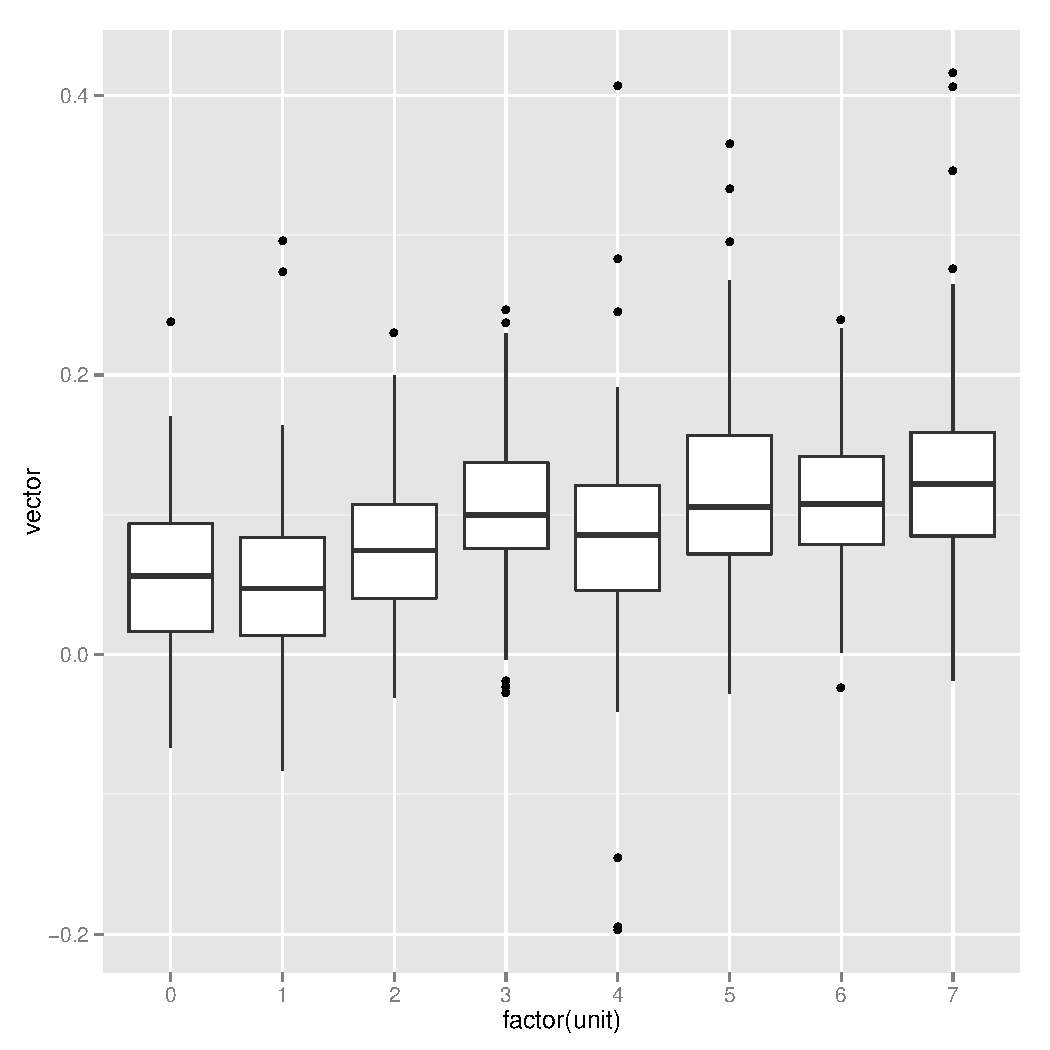
\includegraphics[width=0.7\textwidth,trim= 0 0 20 30, clip]{quizcorrelationbox.pdf}
\end{figure}

\newpage

This figure shows a Box and Whisker plot for every question on a quiz to the unrelated questions on the final.
\begin{figure}[h!]
    \centering
    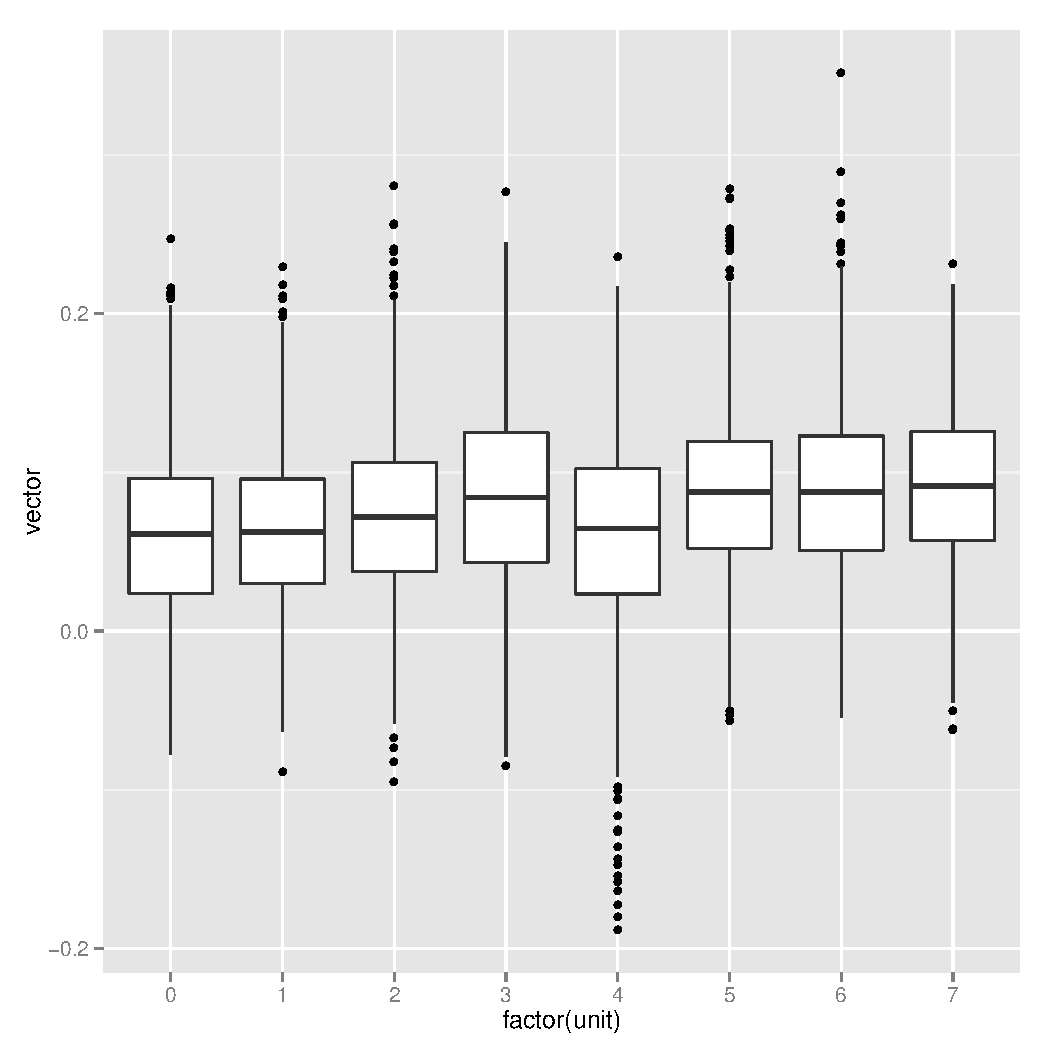
\includegraphics[width=0.7\textwidth,trim= 0 0 20 30, clip]{unrelatedcorrelationbox.pdf}
\end{figure}
\FloatBarrier

\newpage

This figure shows the mean correlations of quiz questions on related and unrelated questions on the final side by side.
\begin{figure}[h!]
    \centering
    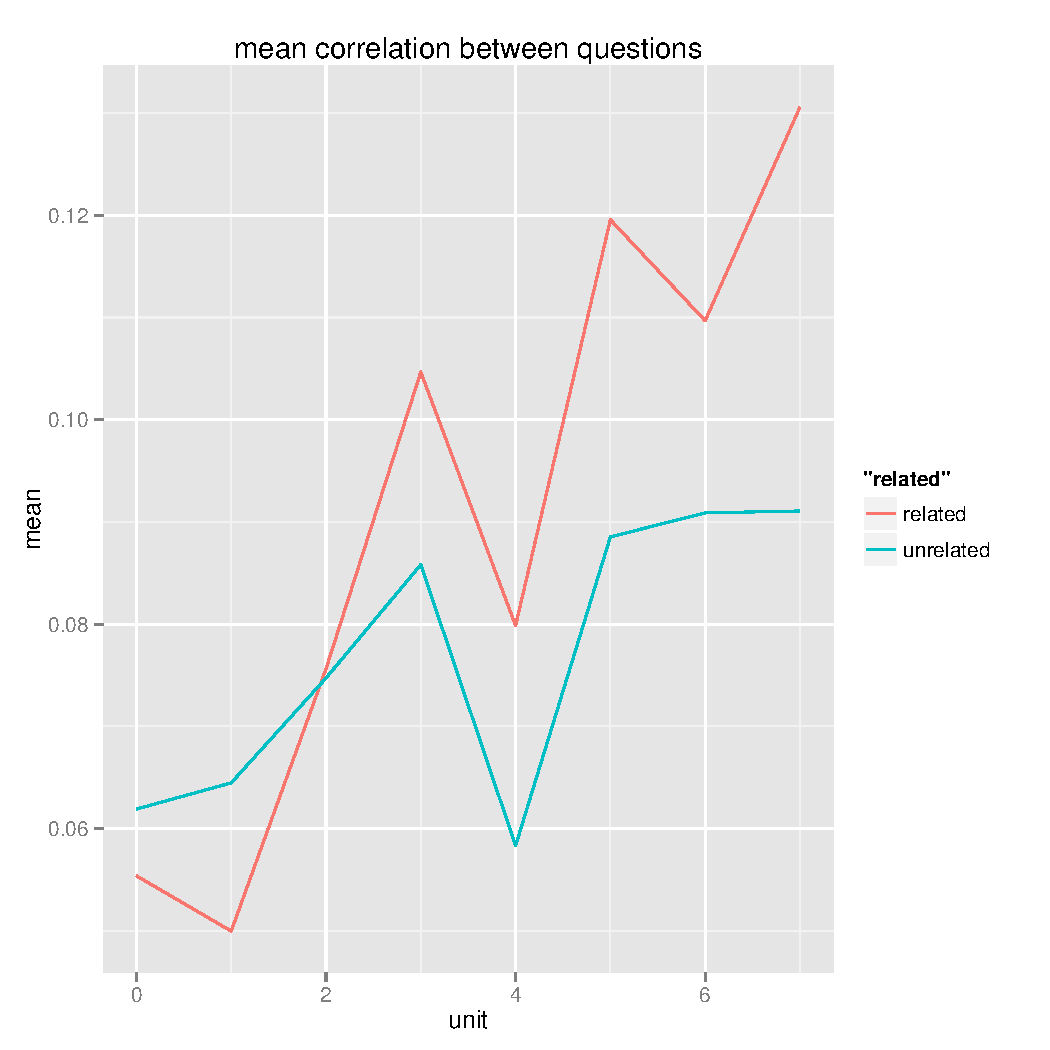
\includegraphics[width=0.7\textwidth,trim= 0 0 20 30, clip]{correlationlines.pdf}
\end{figure}
\FloatBarrier


\subsection{Conclusions}
\subsubsection{Correlations}
Judging from the graphs provided, the correlation of quiz scores with the final had a few interesting trends. One was an outcome we expected, which is that quizzes later in the course more strongly correlate with their questions on the final, most likely due to the simple fact that the material is fresher in the student's minds. This trend can be seen both in the box plot and in the line graph. \\

Another trend can be seen in the box plots as well: That there are many outliers, expecially later on in the course. The outliers that have much higher correlation are easy to explain because one would expect that questions which are testing the same material woulc have stronger correlations than those testing different material in the same subject. However, there are also outliers in the other direction, even going so far as to have a few questions that are negatively correlated with exam scores. We suspect that this could be due to those being trick questions, that students only studied because they happened to guess wrongly on the quiz, but without having access to the questions themselves, this can at best only be a guess as to why these trends are appearing.

\end{singlespace}
\end{document}
